\documentclass[letterpaper,12pt,twoside,]{pinp}

%% Some pieces required from the pandoc template
\providecommand{\tightlist}{%
  \setlength{\itemsep}{0pt}\setlength{\parskip}{0pt}}

% Use the lineno option to display guide line numbers if required.
% Note that the use of elements such as single-column equations
% may affect the guide line number alignment.

\usepackage[T1]{fontenc}
\usepackage[utf8]{inputenc}

% pinp change: the geometry package layout settings need to be set here, not in pinp.cls
\geometry{layoutsize={0.95588\paperwidth,0.98864\paperheight},%
  layouthoffset=0.02206\paperwidth, layoutvoffset=0.00568\paperheight}

\definecolor{pinpblue}{HTML}{185FAF}  % imagecolorpicker on blue for new R logo
\definecolor{pnasbluetext}{RGB}{101,0,0} %


\usepackage{wrapfig,subcaption,array,tabularx,multirow,caption} \usepackage[utf8]{inputenc}

\title{QBUS2820 Assignment2}

\author[a]{SID: 480110301}


\setcounter{secnumdepth}{0}

% Please give the surname of the lead author for the running footer
\leadauthor{}

% Keywords are not mandatory, but authors are strongly encouraged to provide them. If provided, please include two to five keywords, separated by the pipe symbol, e.g:
 

\begin{abstract}

\end{abstract}

\dates{This version was compiled on \today} 

% initially we use doi so keep for backwards compatibility
% new name is doi_footer

\pinpfootercontents{QBUS2820 Assignment 2}

\begin{document}

% Optional adjustment to line up main text (after abstract) of first page with line numbers, when using both lineno and twocolumn options.
% You should only change this length when you've finalised the article contents.
\verticaladjustment{-2pt}

\maketitle
\thispagestyle{firststyle}
\ifthenelse{\boolean{shortarticle}}{\ifthenelse{\boolean{singlecolumn}}{\abscontentformatted}{\abscontent}}{}

% If your first paragraph (i.e. with the \dropcap) contains a list environment (quote, quotation, theorem, definition, enumerate, itemize...), the line after the list may have some extra indentation. If this is the case, add \parshape=0 to the end of the list environment.


\captionsetup[figure]{labelfont={it,bf,scriptsize},textfont={it,scriptsize},labelsep=colon}
\captionsetup[table]{labelfont={it,bf,scriptsize},textfont={it,scriptsize},labelsep=colon}
\captionsetup[FLOAT_TYPE]{labelformat=simple, labelsep=colon}

\hypertarget{task-a}{%
\section{Task A}\label{task-a}}

\hypertarget{introduction}{%
\section{Introduction}\label{introduction}}

In a traditional manner, sale prices of houses were predicted by
comparing sale prices and costs in the real estate market. There was no
general standard to estimate the value of houses. Machine learning
techniques therefore play an important role to help establishing models
for sale prices of house predictions. It has been stated that the
availability of a house price prediction model helps fill up an
essential information gap and improve the efficiency of the real estate
market (Calhoun, 2003).

This project aims to develop predictive models for sale prices of house
with machine learning techniques. With the sale price which is a
numerical variable being the response of predictive models, five models
are developed and validated.

By comparing the root mean squared errors of predictions, the lasso
regression model and random forest model are found to have the best
predictive performance for the housing data, compared to elastic net,
ridge regression, k-nearest neighbor regression and stepwise regression
with forward selection.

\hypertarget{data-processing-and-exploratory-data-analysis}{%
\section{Data processing and exploratory data
analysis}\label{data-processing-and-exploratory-data-analysis}}

There are 36 numeric variables and 43 categorical variables in the
housing data. By calculating the correlation coefficient, 12 numeric
variables are found to be highly linearly related to sale price, as the
absolute values of corresponding correlation coefficients are greater
than 0.5. The distributions of these variables are visualized in figure
\ref{fig:scatter}. `TotRms AbvGrd', `Garage Area', `1st Fir SF' and
`SalePrice' are shown to be right-skewed while `Garage Yr Blt' and
`Overall Qual' are left-skewed, but these distributions are
significantly influenced by outliers in several columns. Moreover, some
variables, such as `TotRms AbvGrd', tend to have linear relationships
with other variables except sale price, leading to multi-collinearity.
This could violate the assumption of some predictive models, such as
multiple linear regression, thus robustness to multi-collinearity should
be carefully considered when developing predictive models.

Figure \ref{fig:boxplots} shows the distribution of sale price with
regard to different categorical features. For most categorical features,
sale prices tend to largely different for different groups of the
categorical feature, except `BsmtFin Type 2' and `Land Slope'. However,
although medians sale prices look similar for different groups of
`BsmtFin Type 2' and `Land Slope', the distribution of sale prices are
not identical. Hence, it can still be worthwhile to include these two
variables as features to predict sale price. In addition, the boxplots
also highlight the outliers of sale price existing in different
categorical groups.

Besides affecting the shapes of data distribution, the existing outliers
of numeric variables can also post an effect on predictive performance
and goodness of fit of models. However, as long as these outliers do not
violate the assumptions of predictive models, it is acceptable to
contain outliers when developing models.

\hypertarget{feature-engineering}{%
\section{Feature engineering}\label{feature-engineering}}

\begin{wrapfigure}{r}{0.5\textwidth}
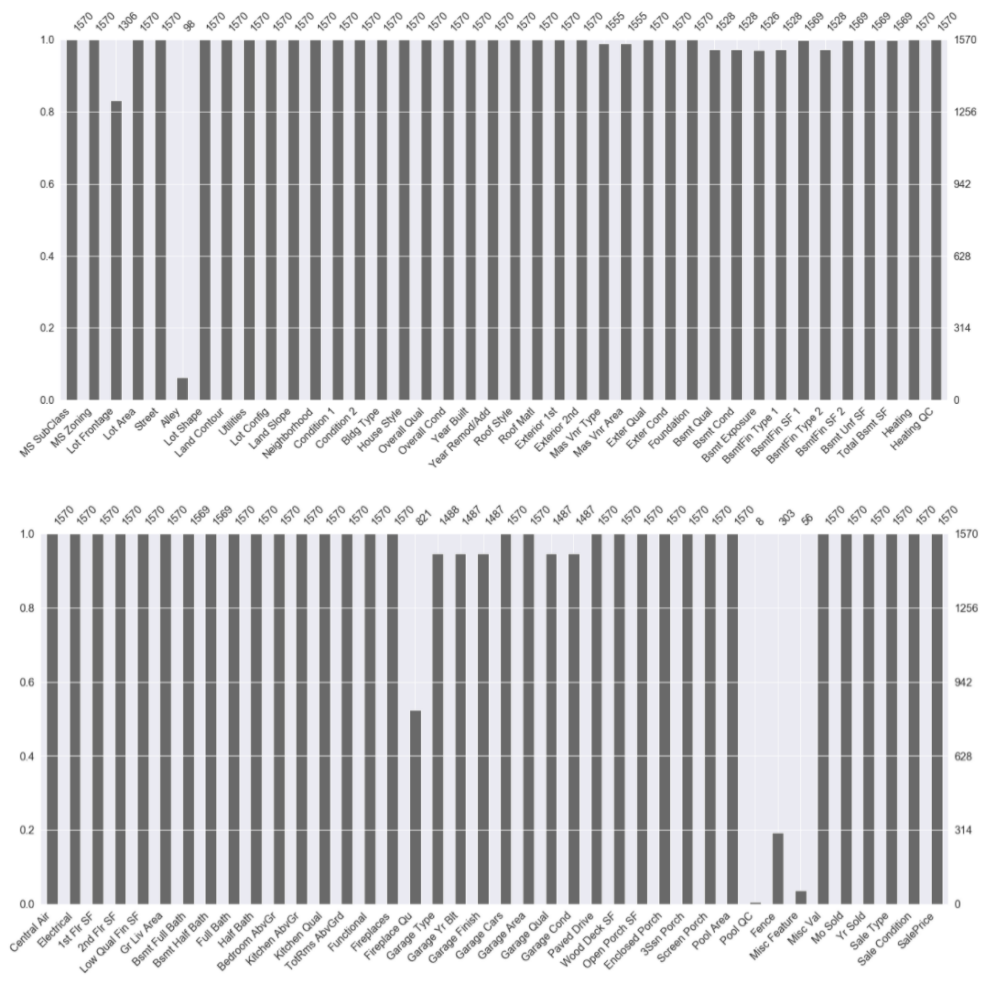
\includegraphics[width=1\linewidth]{miss_plot.png}
\centering
\caption{Visualizing missingness of housing data in training set.}
\label{fig:miss}
\end{wrapfigure}

As shown in Figure \ref{fig:miss}, there are huge amounts of missing
values in several columns: `Alley', `Fireplace Qu', `Pool QC', `Fence',
`Misc Feature', with more than 40\% missing values within each column.
With this issue, such variables are uninformative to be a feature of
predictive models as there are too few observations. To deal with this,
removing all rows with missing values can lead to significant loss of
information, while imputation using small amount of observations can
misrepresent the population for largely incomplete columns. Therefore,
`Alley', `Pool QC', `Fence', `Misc Feature' are abandoned due to high
missing rates.

Besides, there are 19 columns containing missing values but the
percentages of missing values are less than 20\%. This can be deal with
by imputation. The missing values are imputed by using the most frequent
value of each column.

From exploratory data analysis, the numeric variables tend to have
different scales. Therefore, data standardization is performed prior to
model development for numeric variables by subtracting the mean,
followed by dividing the standard deviation of the corresponding
columns.

After feature engineering, there are 74 informative features, with 36
features being numeric and 38 features being categorical. There are 1570
observations in the training set and 1210 observations in the testing
set. For regression models involving categorical features, dummy
variables are created for each categorical feature.

\hypertarget{methodology}{%
\section{Methodology}\label{methodology}}

Five regression models are trained by two sets of data where one
training set contains numeric features only and the other set includes
both categorical and numeric features. With regards to the issue of
multi-collinearity mentioned before, all of the five regression
techniques used are capable for addressing multi-collinearity. Therefore
there is no need to eliminate features suffering from
multi-collinearity, and all features surviving in the feature
engineering stage are involved in predictive models development.

To develop the best parameter set for each regression models,
hyperparameters are tuned with 5-fold cross validation. The performance
of models with different values of hyperparameters is estimated by
negative mean squared error, where a larger score indicates better
predictive performance. For each machine learning model, the value of
hyperparameter resulting in the best performance is selected to be
optimal.

\hypertarget{random-forest-regression}{%
\subsection{Random forest regression}\label{random-forest-regression}}

A random forest regression model, which is an extension of decision
tree, is developed. It is a supervised learning techniques is developed.
which applies ensemble learning method for regression. With this
technique, decision trees are created in parallel by bagging
(i.e.~reduce the variance of predictions by resampling). In this case,
the mean predicted sale price of the individual trees is reported.

As random forest applies bootstrap sampling, multi-collinearity is not a
concern because it is simply selecting different features from training
set to develop models. In addition, the splits of each tree are randomly
sampled from the training set so that with the randomness, overfitting
can be avoided.

The number of features being spitted on at each leaf node which is a
hyperparameter is the main focus to find the optimal random forest
model. Another determinant parameter is the number of trees in random
forest. To tun the random forest model, 10 values, which are 200, 400,
600, 800, 1000, 1200, 1400, 1600, 1800 and 2000, for number of trees
(`n\_estimators') are fed into models. The maximum number of features
being spitted, which is presented as `max\_feature' in python, is
obtained by taking a square root of the number of feature.

The optimal number of features being spitted is 1200 for the training
set with numeric features only. The optimal number changes to 200 when
the model involves both categorical and numeric features. By design, the
random forest model is a black box method, making it hard to interpret
compared to other models in this study.

\hypertarget{lasso-regression}{%
\subsection{Lasso Regression}\label{lasso-regression}}

A lasso regression model is developed as it is able to deal with
multi-collinearity as well as feature selection. As such it is a highly
automate technique with satisfactory predictive performance and
interpretability.

The key component of the lasso model is to perform L1 regularization.
Hence the objective is to minimize
\(\sum^n_{i=1}(y_i-\beta_0-\sum_jx_{ij}\beta_j)^2+\lambda\sum^p_{j=1}|\beta_j|\),
where \(\lambda\) is the hyperparameter which is tuned to control the
strength of L1 regularization penalize. Increasing \(\lambda\) results
in higher level of L1 penalty and thus more features are eliminated.
This also affects the bias-variance trade-off as a increase of
\(\lambda\) leads to a increase in bias and a decrease in variance.

It might be challenging to initialize a list of lambdas to tun the model
as there is no strict upper boundary of lambdas. Fortunately, the
\texttt{LassoCV} package in python can fit the data and automatically
find out the optimal \(\lambda\) among 100 different values ranging from
65 to 64990. For the numeric training set, the optimal value of
\(\lambda\) is 921.2 while it is 130.6 for model including both numeric
and categorical features.

36 features are selected by the numeric model, with ``Gr Liv Area'',
``Overall Qual'', ``BsmFin SF 1'', ``Total Bsmt SF'' and ``Misc Val''
being the top 5 significant predictors for sale price of house. 98
features are selected by the model involving numeric and categorical
features while ``Roof Matl\_WdShngl'', ``Exter Qual\_Ex'',
``Neighborhood\_NoRidge'', ``Neighborhood\_NridgHt'' and ``Gr Liv Area''
constribute the most to predict sale price.

\hypertarget{ridge-regression}{%
\subsection{Ridge Regression}\label{ridge-regression}}

A ridge regression which is similar with the lasso regression, is
constructed. In stead of L1 regularization, the ridge regression applies
L2 regularization which does not help selecting features but it can
still overcome the issue of multi-collinearity.

The hyperparameter is \(\lambda\), being similar with that of lasso
regression, to minimize
\(\sum^n_{i=1}(y_i-\beta_0-\sum_jx_{ij}\beta_j)^2+\lambda\sum^p_{j=1}\beta_j^2\).
The \texttt{RidgeCV} package in python helps to fit data and select the
optimal value of lambda from 100 values. The optimal lambdas for numeric
training set and full training set are 113.2 and 9.6 respectively, which
are largely different.

\hypertarget{elastic-nets}{%
\subsection{Elastic Nets}\label{elastic-nets}}

An elastic nets model performs both L1 and L2 regularization, and
integrates the strength of ridge regression and lasso regression. As
such, it is able to perform certain level of feature selection as well
as placing no restriction on the number of selected variables.

The hyperparameter \(\lambda\) is tuned to minimize
\(\sum^n_{i=1}(y_i-\beta_0-\sum_jx_{ij}\beta_j)^2+\lambda\sum^p_{j=1}(\alpha \beta_j^2+(1-\alpha)|\beta_j|)\).
Being similar to \texttt{RidgeCV} and \texttt{LassoCV}, the
\texttt{ElasticNetCV} package in python selects the optimal value of
\(\lambda\) from 100 different values for the fitted data. The optimal
lambdas are both 65.6 for numeric set and full set.

\hypertarget{stepwise-regression}{%
\subsection{Stepwise regression}\label{stepwise-regression}}

The stepwise regression is simply a multiple linear regression with
feature selection. The forward selection approach starts from a null
model which contains only the constant, and iterate to add different
number of features to the model. For each iteration, all predictors are
add individually to the model to construct \(p-k-1\) models, where \(p\)
is the total number of predictors available, and \(k\) is the number of
predictors involved in models. For a specific value of \(k\), the best
model is selected based on residual sum of square (RSS). Finally, the
optimal stepwise model is selected by comparing the negative root mean
squared error from cross validation, in order to estimate predictive
performance of models involving different number of predictors.

The optimal model with numeric features contains 17 predictors while the
best model including both categorical and numeric variables contains 73
features.

\hypertarget{cross-validation-results}{%
\section{Cross validation results}\label{cross-validation-results}}

\begin{wraptable}{r}{8cm}
\begin{tabular}{ |c|c|c| } 
\hline
\textbf{Model / Features} & \textbf{Numeric} & \textbf{Numeric and Categorical} \\
\hline
\textbf{Forward stepwise} & 34470.77 & $5.21\times 10^{15}$ \\ 
\textbf{Lasso} & 34543.61 & 29628.07 \\
\textbf{Ridge} & 34475.68 & 30082.79 \\
\textbf{Elastic net} & 35380.58 & 32844.26 \\
\textbf{Random forest} & 28006.66 & 28797.24\\
\hline
\end{tabular}
\centering
\caption{Summary of predictive performance for regression models. The performance assessment metric is the root mean squared error from cross validation.}
\label{table:cv_errors}
\end{wraptable}

The predictive performance of models developed are validated by root
mean squared error (RMSE) from 5-fold cross validation. Table
\ref{table:cv_errors} summaries the predictive performances of five
regression models for the two training sets. For models including only
numeric features, random forest regression has the best performance with
the lowest RMSE while other 4 models have similar performance. For
models with both numeric and categorical variables, random forest
regression still has the most accurate predictions, followed by lasso
regression.

It is noticeable from table \ref{table:cv_errors} that the stepwise
regression with forward selection has a poor predictions with a very
large RMSE for training set involving categorical variables, whereas the
predictive performance for numeric set is relatively satisfactory. This
is because when performing stepwise regression, the dummy variables with
values of 0 and 1 are treated as numeric variable when fitting multiple
linear regression. This can pose a detrimental influence on predictive
performance when forward selection does not handle this issue.

\hypertarget{validation-set-results-from-kaggle}{%
\section{Validation set results from
kaggle}\label{validation-set-results-from-kaggle}}

\begin{wraptable}{r}{8cm}
\begin{tabular}{ |c|c|c| } 
\hline
\textbf{Model / Features} & \textbf{Numeric} & \textbf{Numeric and Categorical} \\
\hline
\textbf{Forward stepwise} & 40672.34  & 46984.44 \\ 
\textbf{Lasso} & 39910.50 & 29628.07 \\
\textbf{Ridge} & 40141.87 & 38481.91 \\
\textbf{Elastic net} & 38249.77 &  37679.12\\
\textbf{Random forest} & 25405.28 & 28276.96\\
\hline
\end{tabular}
\centering
\caption{Summary of validation set results from kaggle. The performance assessment metric is the root mean squared error from cross validation.}
\label{table:kaggle_results}
\end{wraptable}

Table \ref{table:kaggle_results} summarizes the validation set results
from kaggle, assessing the predictive performance of five regression
models by root mean squared errors. It is inline with table
\ref{table:cv_errors} that random forest and lasso model regression have
the best predictive performance for both training sets. Moreover, random
forest tends to have more accurate predictions for numeric sets compared
to models with both categorical and numeric variables.

\hypertarget{conclusion-and-discussion}{%
\section{Conclusion and discussion}\label{conclusion-and-discussion}}

In conclusion, regardless of whether including categorical variables,
lasso regression and random forest regression has the best predictive
performance in terms of root mean squared error. Furthermore, lasso
regression, ridge regression and elastic net regression tend to perform
better with both categorical and numeric features while forward stepwise
and random forest regression work better with numeric features.

Suggested by the best predictive model, to estimate the sale price of
house, stakeholders should pay more attention to ``Roof Matl\_WdShngl'',
``Exter Qual\_Ex'', ``Neighborhood\_NoRidge'', ``Neighborhood\_NridgHt''
and ``Gr Liv Area''.

As discussed before, the forward stepwise regression performs poorly
when involving both categorical and numeric feature. This raises a
limitation that it might be inappropriate to include categorical
variables in stepwise regression. Furthermore, outliers can pose a
significant effect on both predictive performance and goodness of fit,
but the potential effect of outliers is not evaluated in the study. To
extend this study, further study could crave for evaluating the
influence of outliers in performance of predictive models by filtering
outliers or applying logarithm transformation. In addtion, to estimate
how categorical affect the sale price of house, ANOVA and might help in
further study. With integration of categorical and numeric features,
random forest and support vector machine can be potential candidates.

\newpage

\hypertarget{appendix}{%
\section{Appendix}\label{appendix}}

\begin{figure}[h]
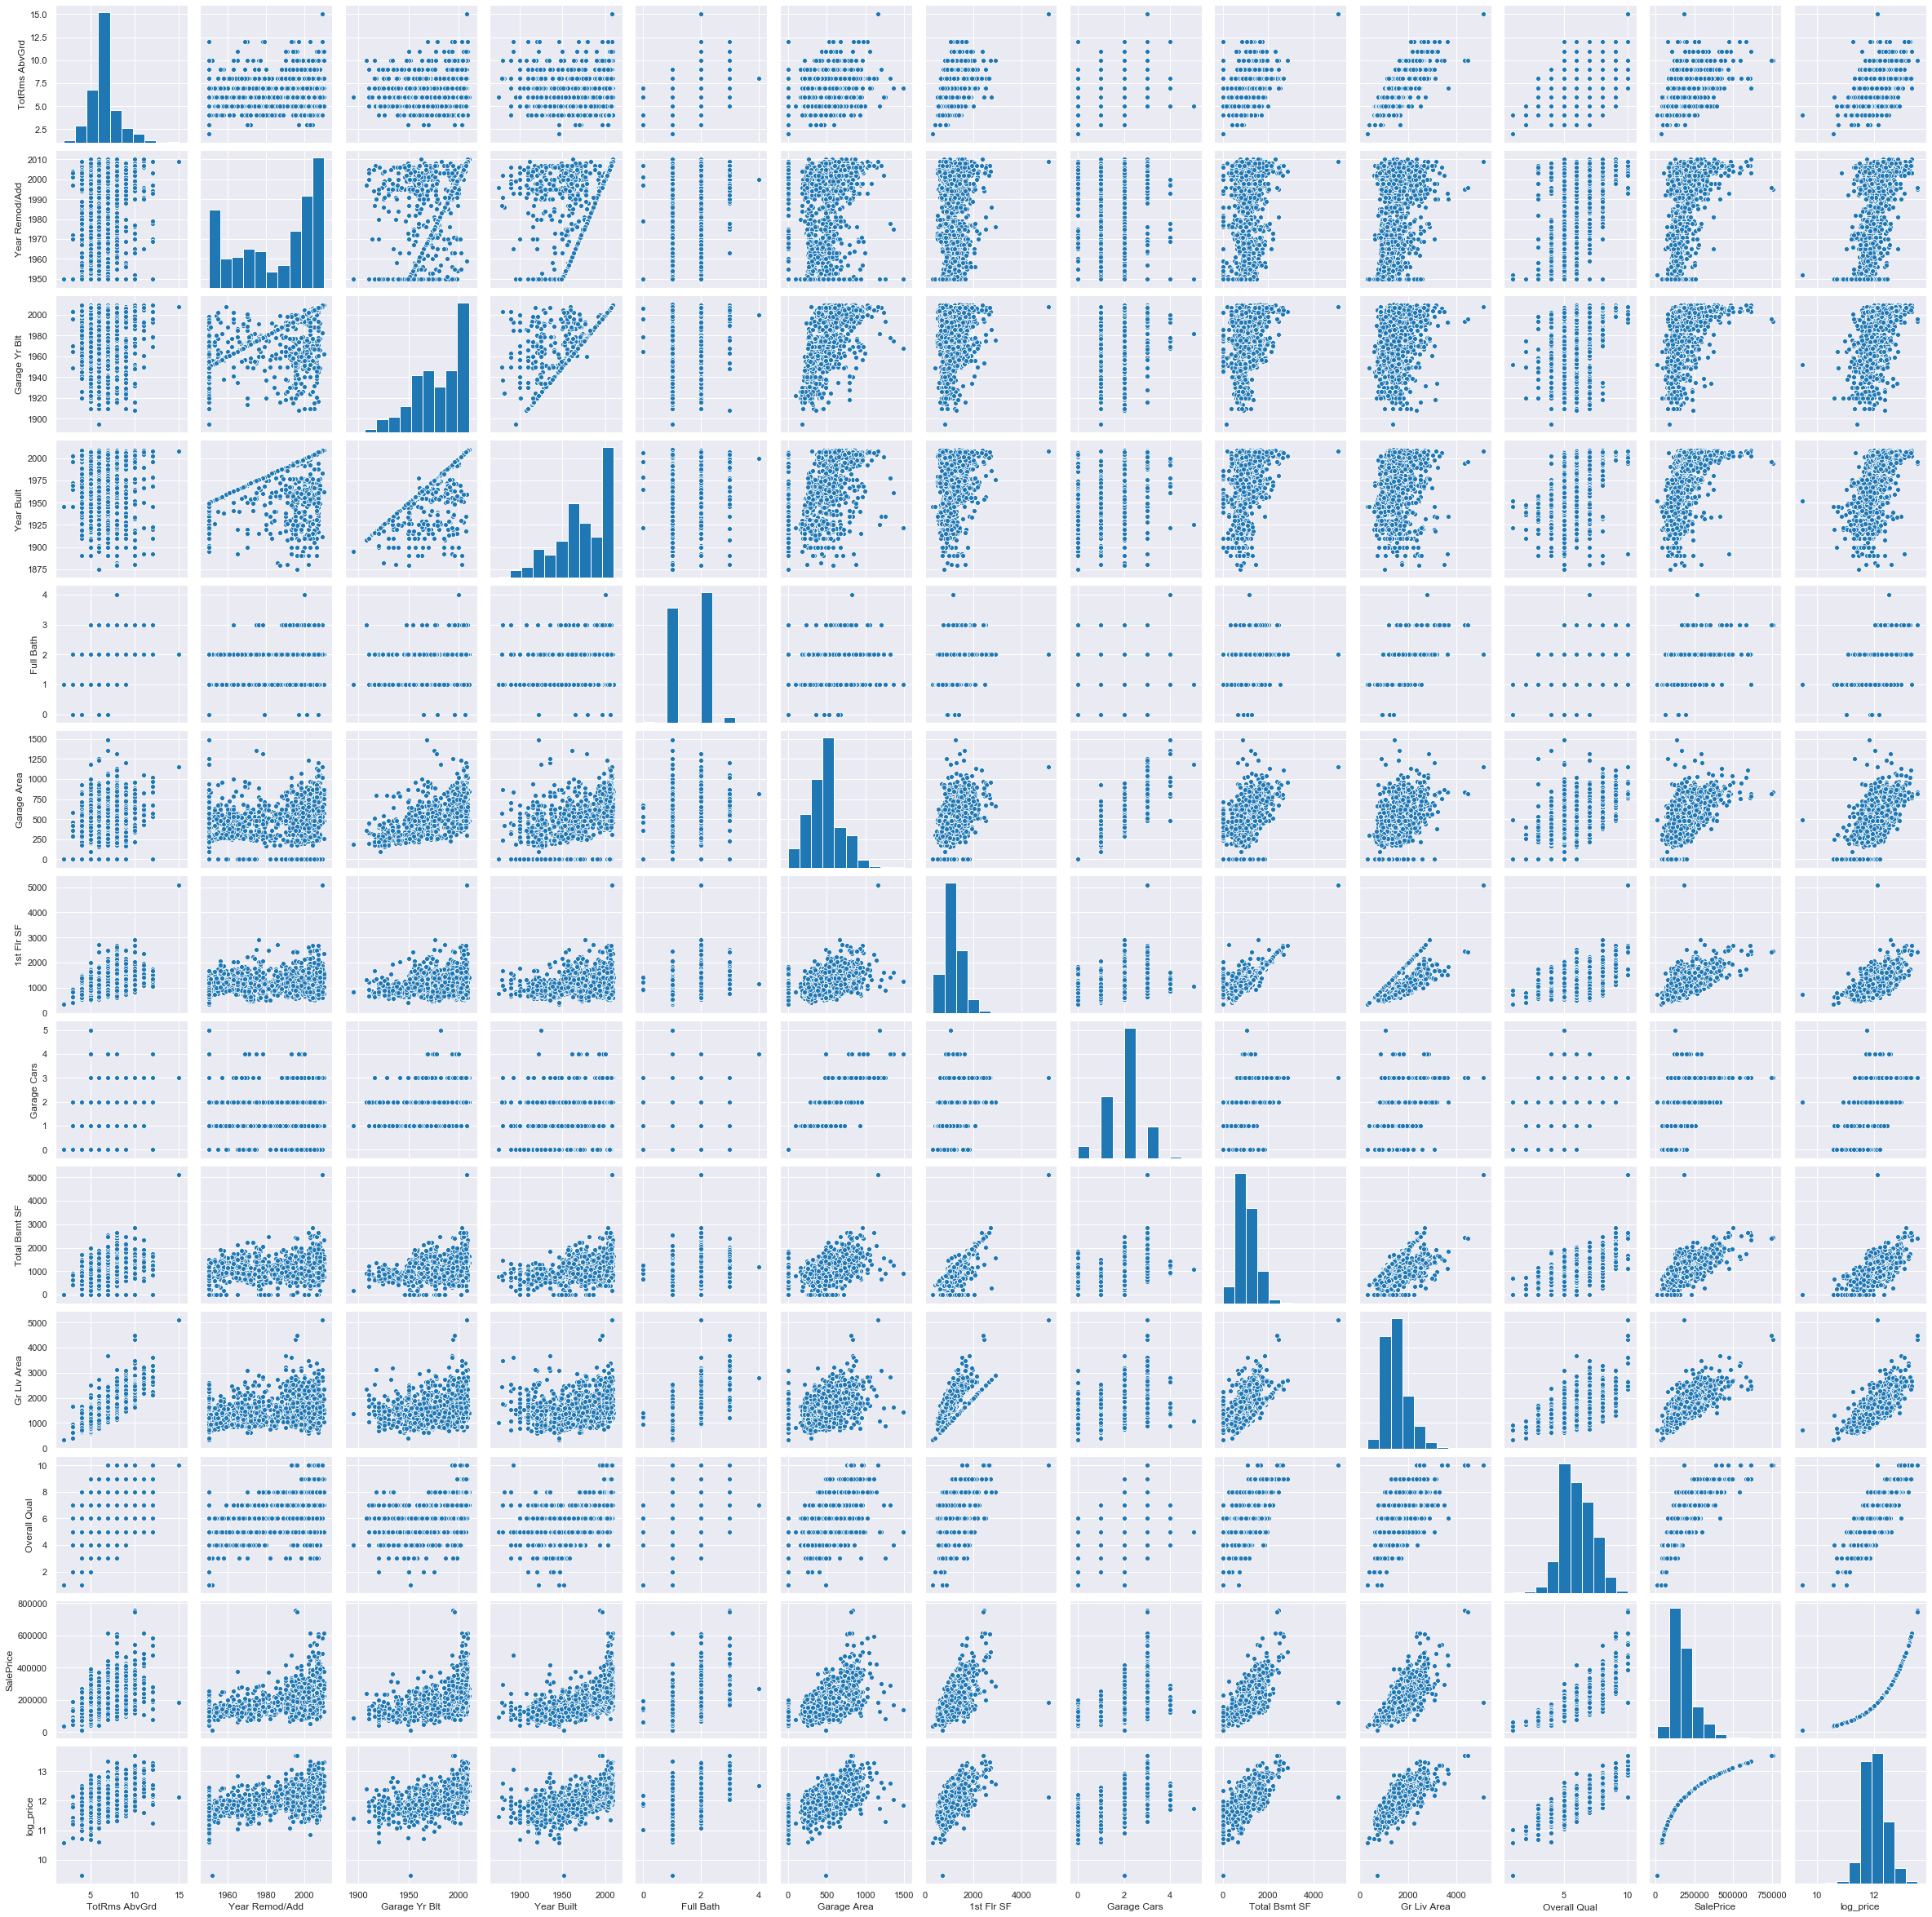
\includegraphics[width=0.8\textwidth]{scatter.png}
\centering
\caption{Distribution of numeric variables in housing data.}
\label{fig:scatter}
\end{figure}

\begin{figure}[h]
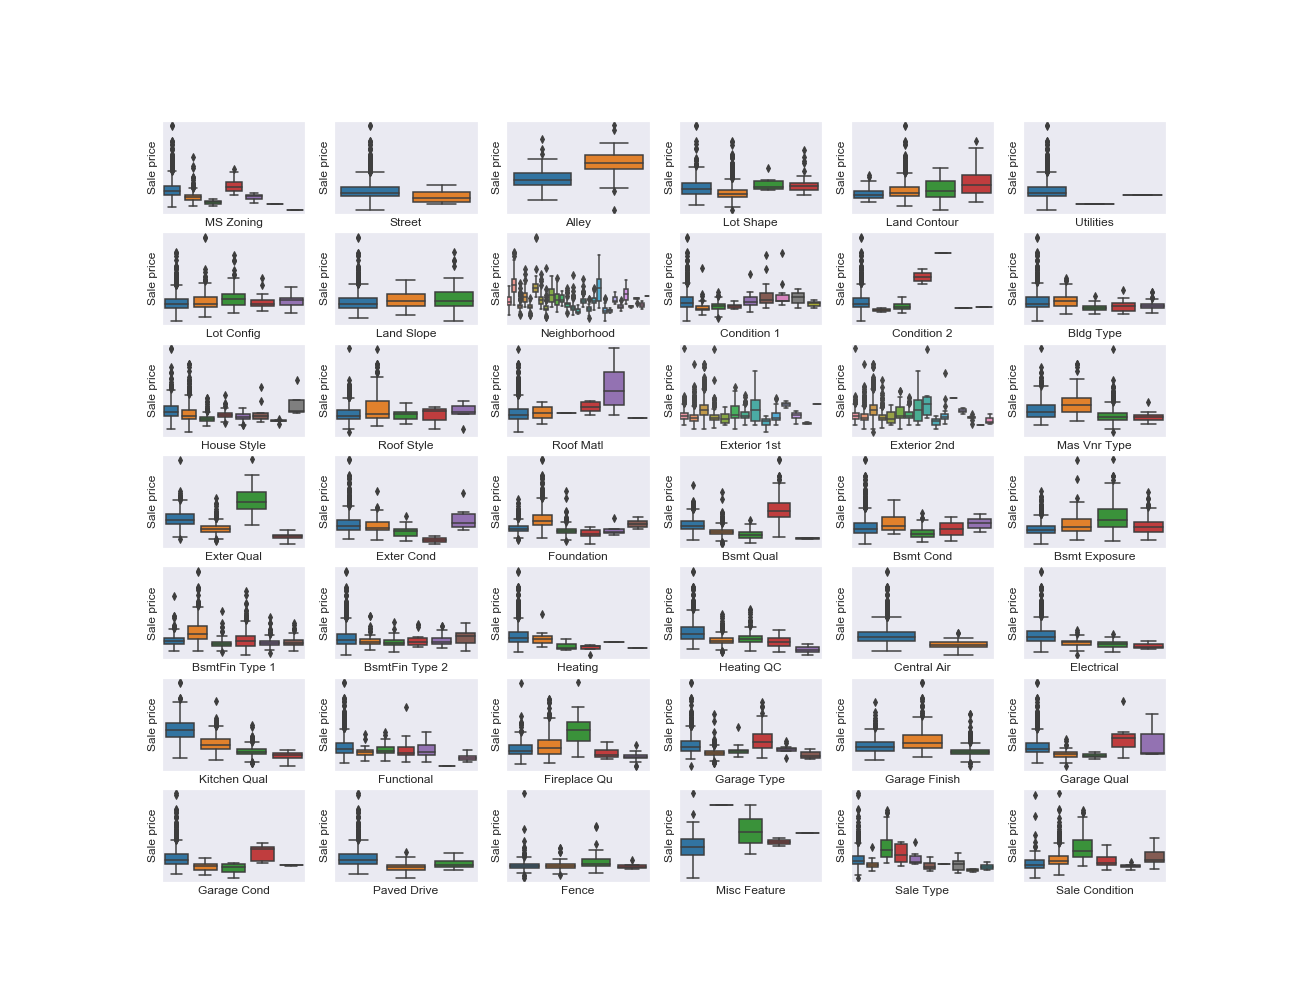
\includegraphics[width=0.8\textwidth]{boxplot.png}
\centering
\caption{Boxplots demonstrating distribution of sale price for houses with different categorical features in housing data.}
\label{fig:boxplots}
\end{figure}

\newpage

\hypertarget{references}{%
\section{References}\label{references}}

\begin{itemize}
\tightlist
\item
  Gibson, M., Little, R. and Rubin, D., 1989. Statistical Analysis with
  Missing Data. The Statistician, 38(1), p.82.
\item
  Scikit-learn.org. 2020. 6.4. Imputation Of Missing Values ---
  Scikit-Learn 0.23.2 Documentation. {[}online{]} Available at:
  \url{https://scikit-learn.org/stable/modules/impute.html}.
\item
  Scikit-learn.org. 2020. 6.4. Imputation Of Missing Values ---
  Scikit-Learn 0.23.2 Documentation. {[}online{]} Available at:
  \url{https://scikit-learn.org/stable/modules/impute.html}.
\item
  Hintze, J.L., 1992. Chapter 335: Ridge Regression. In Number cruncher
  statistical system: statistical software. Kaysville, UT: Jerry L.
  Hintze.
\item
  Chakon, O. (2017). Practical Machine Learning: Ridge Regression Vs
  Lasso. Coding Startups: Coders With Entrepreneurial Mindset. Published
  August 3rd, 2017.
\item
  Allison, P. (2012). When Can You Safely Ignore Multicollinearity?
  Statistical Horizons.
\item
  Cross Validated. (2015). What is elastic net regularization, and how
  does it solve the drawbacks of Ridge (L2) and Lasso (L1)? {[}online{]}
  Available at:
  \url{https://stats.stackexchange.com/questions/184029/what-is-elastic-net-regularization-and-how-doesitsolve-the-drawbacks-of-ridge/184031\#184031}.
\end{itemize}

\newpage

\hypertarget{task-b}{%
\section{Task B}\label{task-b}}

\hypertarget{exploratory-data-analysis}{%
\section{Exploratory data analysis}\label{exploratory-data-analysis}}

There are 312 observations of number of visitors recorded in the
\texttt{Visitors} data. The number of visitors is recorded once a month
from January 1991 to December 2016. The descriptive statistics of number
of visitors show a mean of at 419407.37 and a range from 161400 to
971800.

\begin{wrapfigure}{r}{0.5\textwidth}
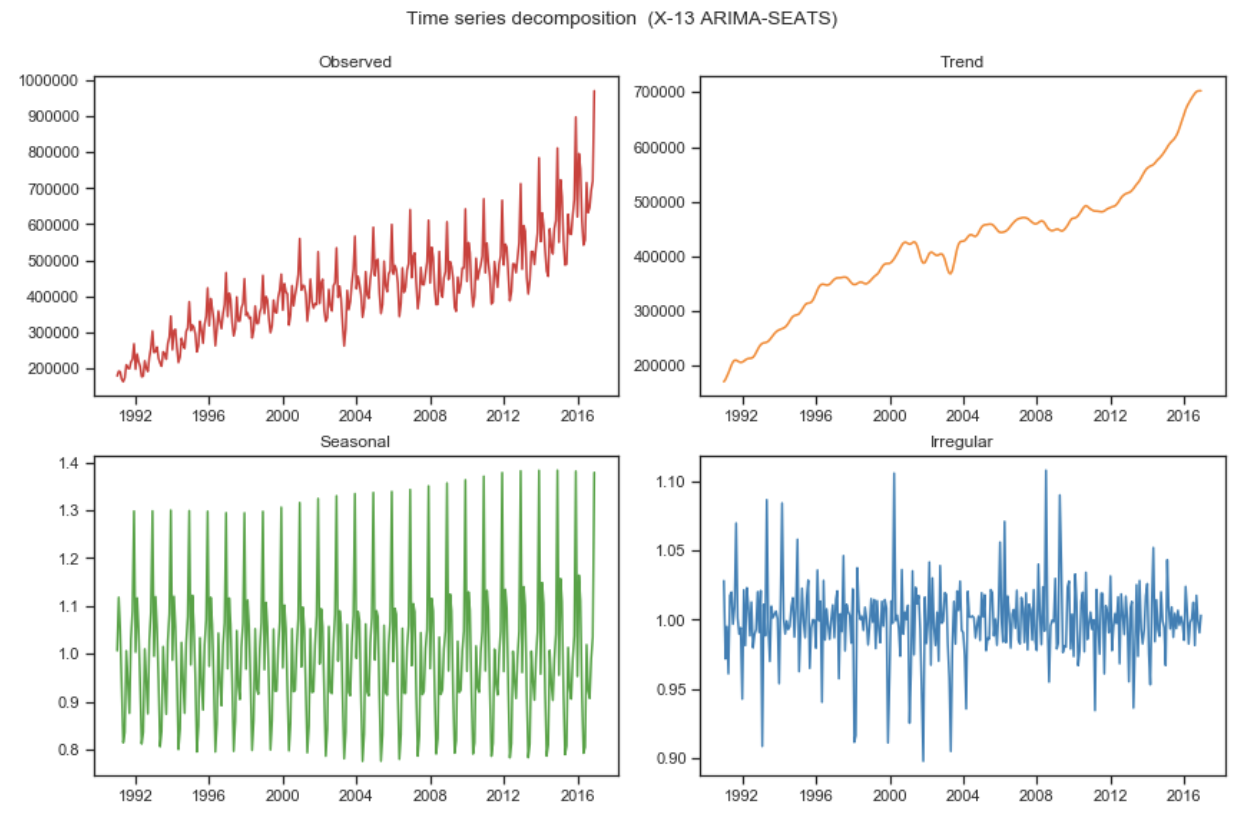
\includegraphics[width=1\linewidth]{decomposition.png}
\centering
\caption{Time series decomposition of number of visitors from 1991 to 2016.}
\label{fig:timeseries}
\end{wrapfigure}

To show the variation of number of visitors through the 25-year period.
Figure \ref{fig:timeseries} shows the time series decomposition of
number of visitors. As systematic changes occur in short periods which
are fixed, it demonstrates an upward trend with a seasonal pattern.
Furthermore, the variation of number of visitors within the fixed period
becomes greater as time moves. As such, a multiplicative forecasting
model may be more suitable for this data compared to an additive model.

\hypertarget{forecasting-models}{%
\section{Forecasting models}\label{forecasting-models}}

To forecast the number of visitors, two exponential smoothing models are
developed.

The basic idea of exponential smoothing is to assign different weights
to recent and past observations by the hyperparamter \(\alpha\). With
the forecast equation

\[\hat y_{t+1}=l_1,\] \[l_t=\alpha y_t+(1-\alpha)t_{t-1}\] where \(l_t\)
represents the level of the time series. A larger \(\alpha\) gives
greater weight to recent observations, and therefore the forecasts are
more adaptive to recent changes in the series. In contrast, a lower
\(\alpha\) assign greater weight to the past observations, making the
forecast smoother.

\hypertarget{holt-winters-exponential-smoothing}{%
\subsection{Holt-Winters exponential
smoothing}\label{holt-winters-exponential-smoothing}}

As an extension of simple exponential smoothing, the Holt-Winters
exponential smoothing capture not only the trend but also the seasonal
pattern of number of visitors. It is available for both additive and
multiplicative models. In this case, as mentioned before, the variance
of number of visitors increases as time goes by, a multiplicative model
is considered.

The model involves three hyperparameters \(\alpha,\beta,\delta\),
ranging from 0 to 1, which control the level, trend and seasonal indices
respectively for the time series of number of visitors. The forecast
equation of a multiplicative model is \[
\hat y_{t+h}=(\hat l_t+h\hat b_t) \times S_{t-L+(h~mod~L)},
\] \[
l_t=\alpha(y_t/S_{t-L}+(1-\alpha)(l_{t-1}+b_{t-1}),
\] \[
b_t=\beta(l_t-l_{t-1})+(1-\beta)b_{t-1},
\] \[
S_t=\delta(y_t/l_t)+(1-\delta)S_{t-L}.
\]

The corresponding objective is, by tuning \(\alpha,\beta,\delta\), to
minimize \[\sum^N_{t=1}(y_t-(l_{t-1}+b_{t-1})\times S_{t-L})^2.\]

\begin{wrapfigure}{r}{0.4\textwidth}
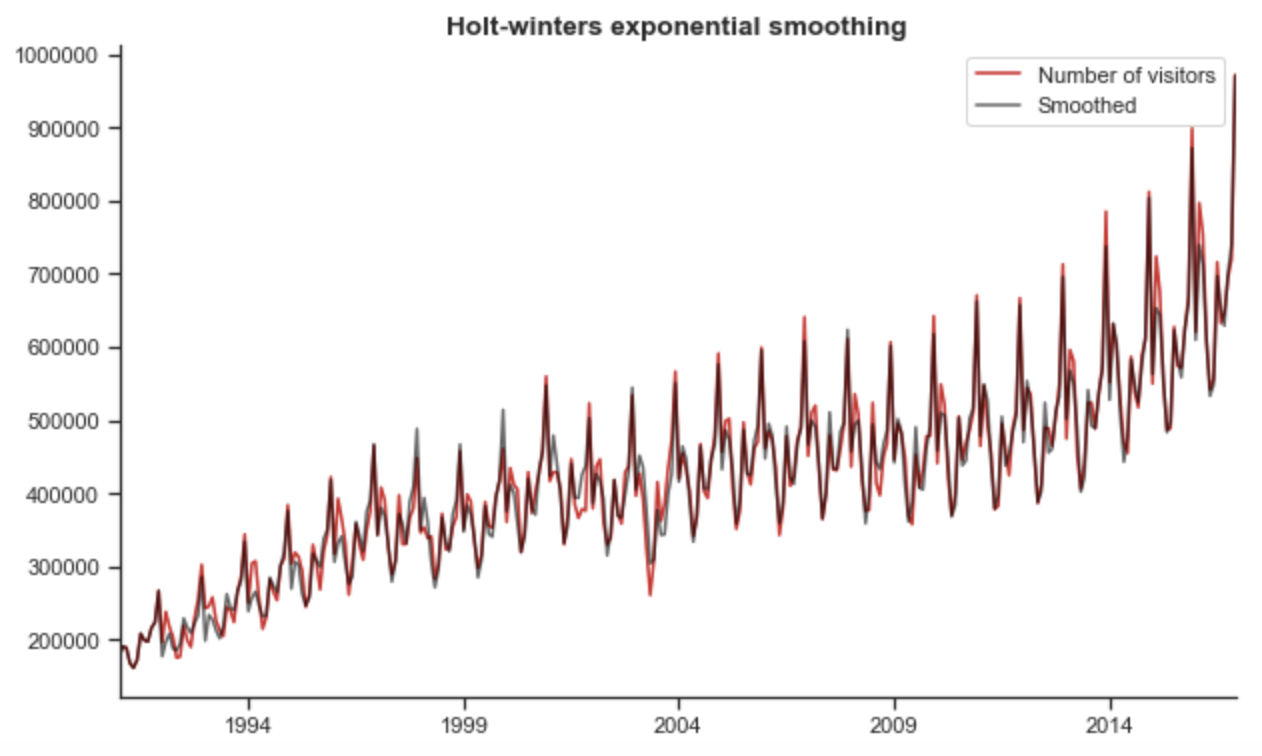
\includegraphics[width=1\linewidth]{HW_es.png}
\centering
\caption{Smoothed time series by Holt-Winter exponential smoothing.}
\label{fig:hw_es}
\end{wrapfigure}

To estimate the appropriate values of hyperparameters,
\(\alpha, \beta,\delta\) are initially set to 0.1, 0.1 and 0.05
respectively, and are fed into the \texttt{minimize} function in python.
This will automatically selects the values of hyperparameters which
generate the smallest residual sum of squared of predictions.

The optimal hyperparameters of Holt-Winters exponential smoothing are
\(\hat\alpha=0.31,\hat\beta=0.012,\hat\delta=0.362\) for this data.
Figure \ref{fig:hw_es} visualizes the smoothed time series by the
optimal values of hyperparameters. The smoothed series which nearly
converge to the actual time series of number of visitors accurately
capture most of the trend and seasonal pattern.

\hypertarget{damped-trend-exponential-smoothing}{%
\subsection{Damped trend exponential
smoothing}\label{damped-trend-exponential-smoothing}}

The damped trend exponential smoothing models seasonal pattern and trend
of time series based on the Holt-Winters model. Additionally, it helps
preventing the potentially implausible forecasts caused by extrapolating
trends indefinitely into future. To do this, the trend is made smaller
and a damping parameter \(\phi\) ranging from 0 to 1 is considered on
top of the Holt-Winters model. The forecast equation of a damped trend
model is \[
\hat y_{t+h}=l_t+\phi b_t+\phi^2b_t+\phi^3b_t+...+\phi^hb_t,
\] \[
l_t=\alpha y_t+(1-\alpha)(l_{t-1}+\phi b_{t-1},
\] \[
b_t=\beta^*(l_t-l_{t-1}+(1-\beta^*)\phi b_{t-1}.
\]

The objective of the model is, by tuning \(\alpha, \beta, \delta\) and
\(\phi\), to minimize \[
\sum^N_{t=1}(y_t-(l_{t-1}+\phi b_{t-1}+\phi^2b_{t-1}+\phi^3b_{t-1}+...+\phi^hb_{t-1}))^2.
\]

\begin{wrapfigure}{r}{0.4\textwidth}
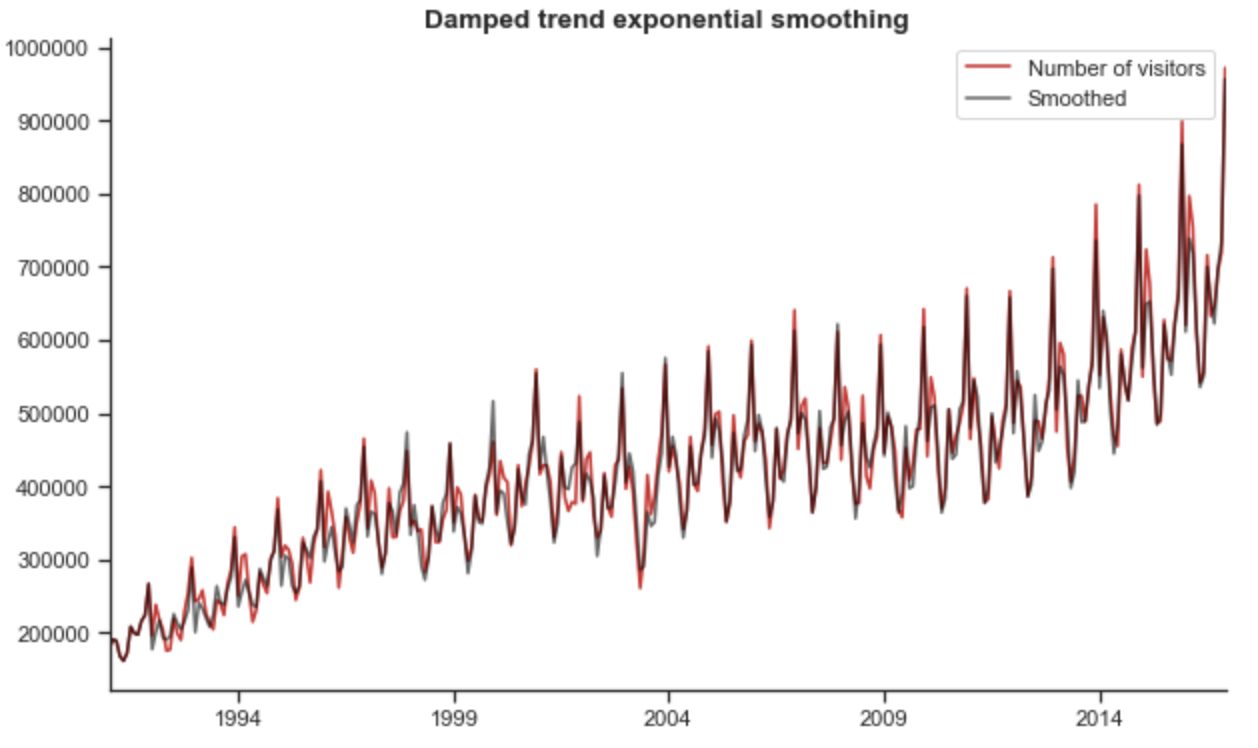
\includegraphics[width=1\linewidth]{damped_smooth.png}
\centering
\caption{Smoothed time series by Holt-Winter exponential smoothing.}
\label{fig:damped_es}
\end{wrapfigure}

To estimate the appropriate values of hyperparameters,
\(\alpha, \beta,\delta,\phi\) are initially set to 0.1, 0.1, 0.05 and
0.98 respectively, and are fed into the \texttt{minimize} function in
python. This will automatically selects the values of four
hyperparameters which generate the smallest residual sum of squared of
predictions.

The optimal values of hyperparameters are
\(\alpha=0.482, \beta=0,\delta=0.413\) and \(\phi=0.792\). Figure
\ref{fig:damped_es} shows the smoothed series of damped trend model
which is highly similar with that of Holt-Winters smoothing. This is
reasonable as two models follow similar rationale to fit models.

\hypertarget{model-diagnostic}{%
\subsection{Model diagnostic}\label{model-diagnostic}}

To check the assumptions of exponential smoothing, residuals are
visualized by four kinds of plots: residual plot, residual
autocorrelation function plot, residual distribution and normal Q-Q
plot. As shown in figure \ref{fig:diag}, with highly similar smoothed
series for Holt-Winters and Damped trend exponential smoothing,
residuals of two models are also similar.

The normal Q-Q plots illustrate a reasonable normal distribution of
residuals as the scatters closely follow the actual Q-Q line excepting a
few outliers. With a large number of observations, the central limit
theorem can be applied, illustrating a normal distribution of data. This
is in line with the distributions of residuals which show a symmetric
bell shape. Moreover, the residual skewness and kurtosis are 0.059 and
0.509 respectively which are small, again proving that the assumption of
normality is satisfied.

The residual plots does not show a clear pattern, representing
homoscedastic variances for both models.

In autocorrelation function plots of residuals, the first coefficient
prominently reach 1, which is reasonable as the first value is comparing
to itself. Other coefficients show a mean at approximately 0
demonstrating relatively low and insignificant sample auto-correlations
in the residual series. This is consistent with a white nose process.

\begin{figure}[h]
\begin{subfigure}{0.5\textwidth}
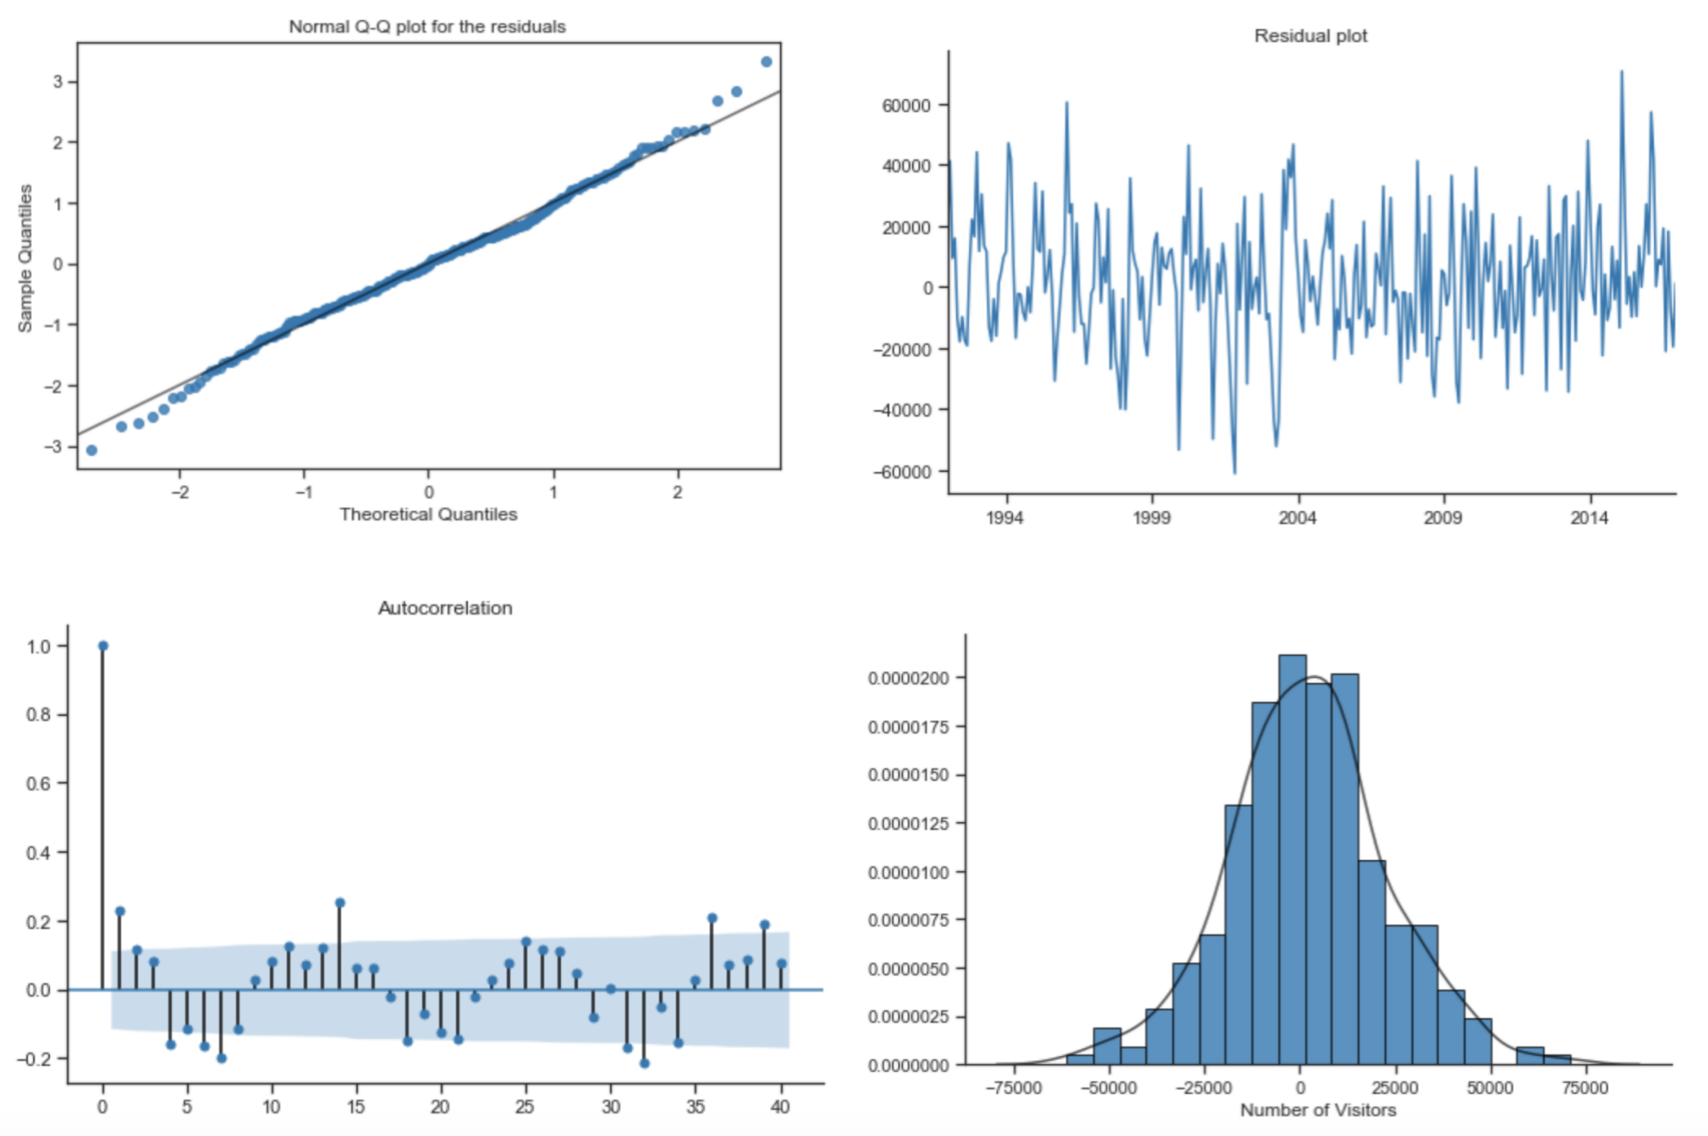
\includegraphics[width=0.9\linewidth, height=5cm]{diagnostic_plot} 
\caption{Holt-Winters exponential smoothing.}
\label{fig:hw_resid}
\end{subfigure}
\begin{subfigure}{0.5\textwidth}
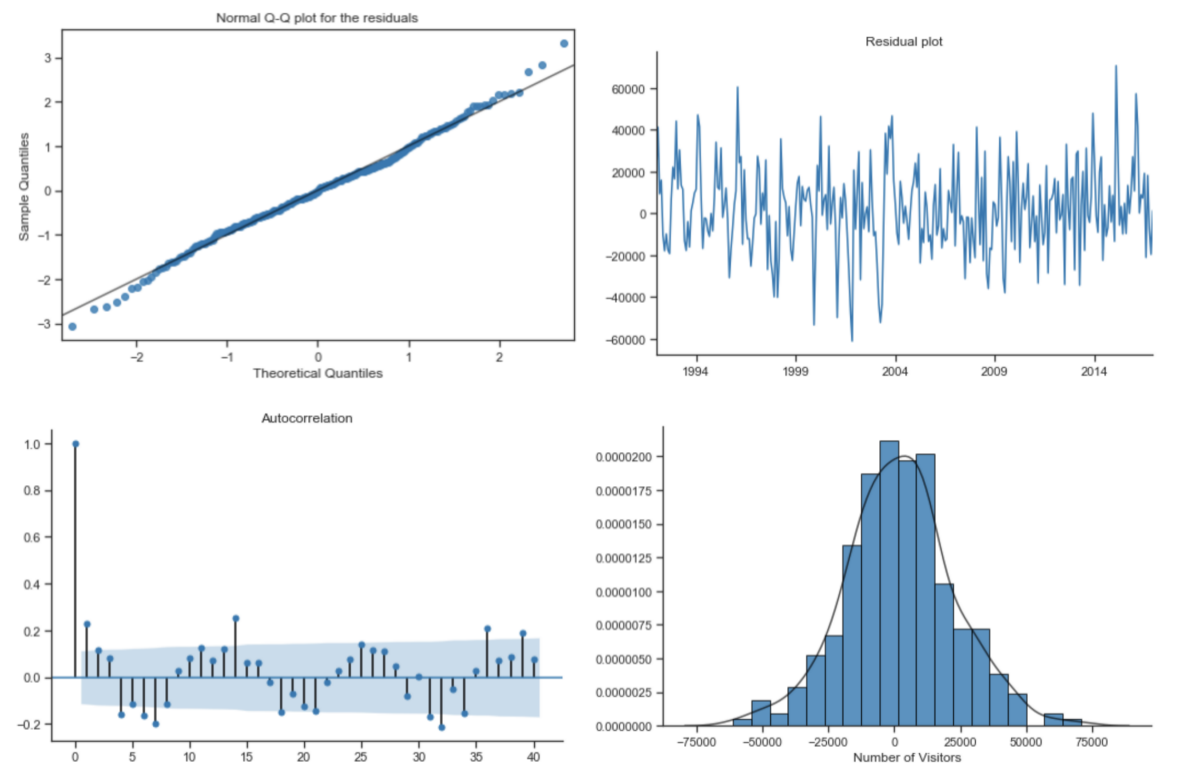
\includegraphics[width=0.9\linewidth, height=5cm]{damped_resid}
\caption{Damped trend exponential smoothing.}
\label{fig:damped_resid}
\end{subfigure}
\caption{Residual plot, residual ACF, residual distribution plot and normal Q-Q plot for exponential smoothing.}
\label{fig:diag}
\end{figure}

\hypertarget{model-validation}{%
\subsection{Model validation}\label{model-validation}}

\begin{wraptable}{r}{8cm}
\begin{tabular}{ |c|c|c| } 
\hline
\textbf{Model / Statistic} & \textbf{RMSE} & \textbf{SE} \\
\hline
\textbf{Holt-Winter} & 23485.87 & 2702.33 \\ 
\textbf{Damped trend} & 24321.72 & 2724.25 \\
\hline
\end{tabular}
\centering
\caption{Summary of predictive performance for number of visitors forecasting by exponential smoothing.}
\label{table:cv_es}
\end{wraptable}

Real time forecasting is performed to validate the predictive
performance of Holt-Winters and damped trend exponential smoothing.
Historical data of number of visitors before January 2010 is used to
train the models. The models developed are then used to forecast the
number of visitors until December 2016. These predictions are compared
to actual historical data to calculate root mean squared errors and
scaled errors.

As shown in table \ref{table:cv_es}, the Holt-Winters model has higher
root mean squared errors and scaled error. This indicates a better
predictive performance for Holt-Winters model compared to damped trend
exponential smoothing. The differences of errors between two models may
result from the ``damped'' trend. As long as the historical data shows a
continuing growing trend, the damped trend predictions tends to be more
deviated to actual data, comparing to the Holt-Winters predictions.

\hypertarget{forecasting-results}{%
\subsection{Forecasting results}\label{forecasting-results}}

The exponential smoothing models forecast the number of visitors for the
following 24 months since the last month in historical data. This
generates predictions for January 2017 to December 2018.

As a simple expression of variance is not available for the
multiplicative Holt-Winters exponential smoothing, it can be challenging
to generate range predictions of number of visitors. Fortunately,
log-additive exponential is basically the same with the multiplicative
models therefore it could be an alternative to make range predictions.

Figure \ref{fig:pred} visualizes the number of visitors predicted by the
two log-additive exponential smoothing models. Both Holt-Winters and
damped trend models forecast the number of visitors to increase and
reach the local maximum nearly in the Christmas holiday, which follows
trend and seasonal pattern for historical data.

To compare the predictions of Holt-Winters and damped trend exponential
smoothing, figure \ref{fig:predictions} shows the point predictions
generated by two models. Although predictions of two models follow a
highly similar seasonal pattern and a growing trend, the predicted trend
of damped trend model is obviously smaller than that of Holt-Winter
model. This is what it means by ``damped'' trend, and it is designed to
prevent implausible forecast by gentling the trend.

\begin{figure}[h]
\begin{subfigure}{0.5\textwidth}
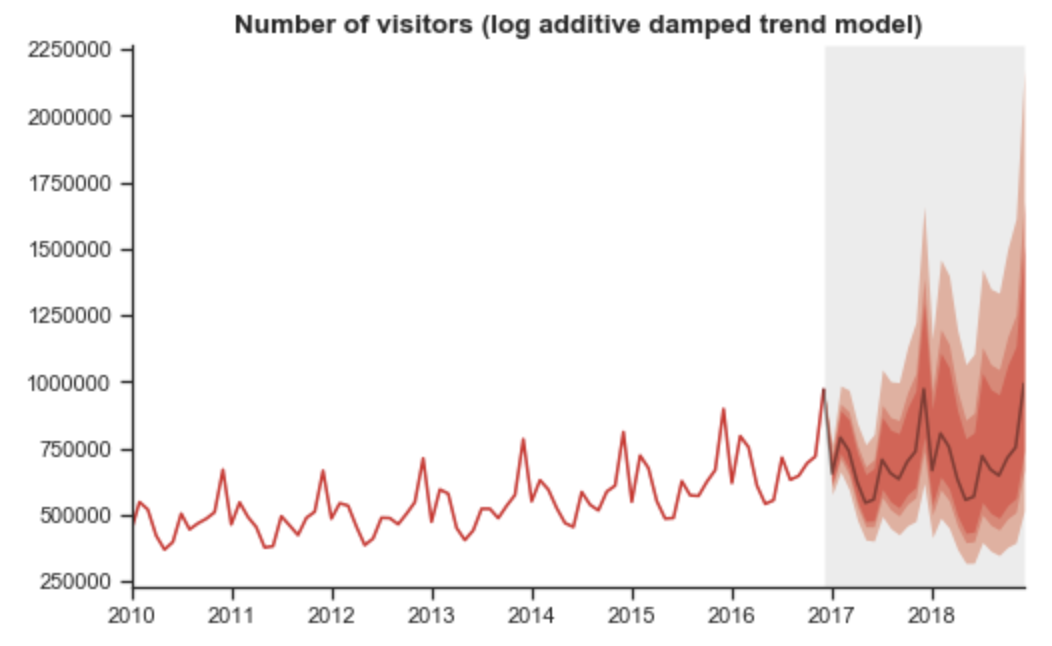
\includegraphics[width=0.9\linewidth, height=5cm]{hw_pred} 
\caption{Holt-Winters exponential smoothing.}
\label{fig:hw_pred}
\end{subfigure}
\begin{subfigure}{0.5\textwidth}
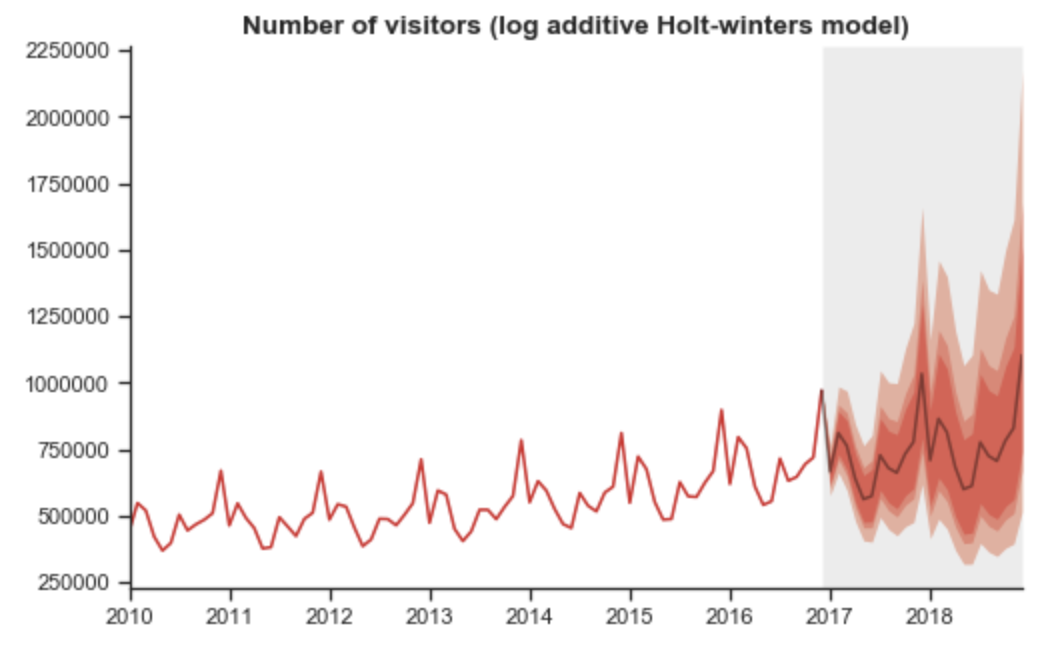
\includegraphics[width=0.9\linewidth, height=5cm]{damped_pred}
\caption{Damped trend exponential smoothing.}
\label{fig:damped_pred}
\end{subfigure}
\caption{Predictions of number of visitors from January 2017 to December 2018.}
\label{fig:pred}
\end{figure}

\begin{figure}[h]
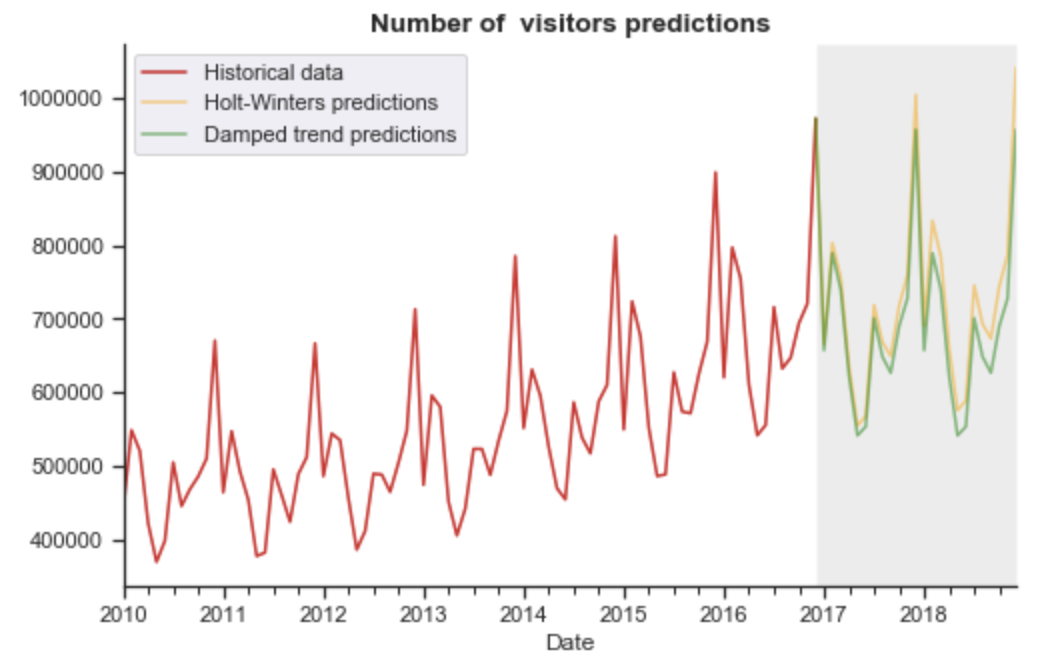
\includegraphics[width=0.6\textwidth]{predictions.png}
\centering
\caption{Point predictions of number of visitors from January 2017 to December 2018 by Holt-Winter and damped trend exponential smoothing. The red, yellow and green lines represent historical data, Holt-Winters predictions and damped trend predictions respectively.}
\label{fig:predictions}
\end{figure}

\hypertarget{conclusion}{%
\section{Conclusion}\label{conclusion}}

To conclude, the number of visitors kept growing with a seasonal pattern
from 1991 to 2016. The seasonal pattern shows that the number of
visitors tends to reach the peak of a year during Christmas holiday. In
addition, the variation between high season and low season in a year was
greater and greater.

Both Holt-Winters and damped trend exponential smoothing predict the
number of visitors to increase in the following two years. The seasonal
pattern of Christmas holiday being the high season is also followed.
Although the two exponential smoothing models generate similar
predictions, damped trend model illustrates a more gentle upward trend
(i.e.~predicted number of customers are smaller) compared to the
Holt-Winters, as it ``damps'' the trend.

%\showmatmethods


\bibliography{pinp}
\bibliographystyle{jss}



\end{document}

